\documentclass{article}

\usepackage[utf8]{inputenc}
\usepackage[T1]{fontenc}
\usepackage[francais]{babel}
\usepackage{graphicx}
\usepackage{hyperref}

\begin{document}
\title{Algorithmes génétiques et application au problème du voyageur de commerce}
\author{Fabien Dubois,\\
   Antoine RATO,\\
   Corentin HEMBISE\\
   \url{https://github.com/dut-info/Algo-Genetique}\\}
\date{\today}

\maketitle

\tableofcontents

\newpage
\section{Principe des algorithmes génétiques}
	\subsection{Introduction}
	Les algorithmes génétiques sont des algorithme qui se basent sur la sélection naturelle afin de trouver des solutions à un problème d'optimisation. 

	La sélection naturelle est un processus de l'évolution des espèces. Les individus les plus adaptés à leur environnement, sont plus susceptible de « survivre », alors au fil de nouvelles générations, la population devient meilleur au regard de son environnement.

	En clair, les algorithmes génétique mime le processus de sélection naturelle pour trouver des solutions efficaces à un problème à un ou plusieurs paramètres.
	Les algorithmes génétiques sont des algorithmes d'approximation puisqu'il ne permettent pas de trouver la solution optimale à un problème, mais de s'en rapprocher. En outre, ils ont l'avantage de trouver une solution en un temps bien inférieur aux algorithmes déterministes.

	Les termes utilisés dans ce genre de problème sont empruntés de la génétique, ainsi, on parlera :
	\begin{description}
	\item [d'individu :] c'est une solution admissible du problème
	\item [de population :] c'est un ensemble d'individus
	\item [de gène :] c'est une partie d'un individu, une partie du problème
	\item [de génération :] c'est une itération de l'algorithme
	\item [de fonction objectif :] c'est une fonction qui permet de définir qu'un individu est meilleur qu'un autre
	\end{description}


	Pourquoi utiliser des algorithmes génétiques ?

	Dans les problèmes d'optimisation où le nombre de variables est grand, 

	\subsection{Principe}
	Les algorithmes de génétique se décomposent en 5 phases :
	\begin{itemize}
	\item La création d'une population initiale
	\item L'évaluation des individus
	\item La sélection des meilleurs individus
	\item Les croisement et les mutations des enfants
	\item La création d'une nouvelle population
	\end{itemize}

	\begin{figure}
		\begin{center}
			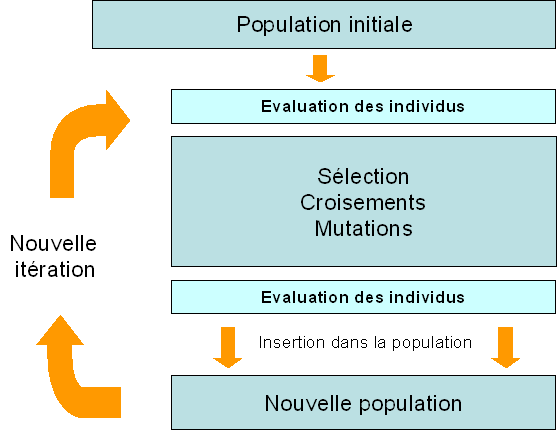
\includegraphics[scale=0.5]{schema_gen.png}
		\end{center}

		\caption{Schéma général d'un algorithme génétique}

		\label{Schéma général d'un algorithme génétique}
	\end{figure}


		\subsubsection{Population initiale}
		La population initiale 
		\subsubsection{Nouveau individus}

\section{Application au porblème du voyageur de commerce}
	\subsection{Définition du problème}
	Le problème est le suivant : 
	\begin{quote}
	Un voyageur de commerce doit visiter $n$ villes données en passant par chaque ville exactement une fois. Il commence par une ville quelconque et termine en retournant à la ville de départ.\\
	Quel chemin faut-il choisir afin de minimiser la distance parcourue ?
	\end{quote}
	
	\subsection{Modélisation du problème}
    Soit :
    \begin{itemize}
        \item $n$ le nombre de villes
        \item $\{v_{i}\}^{n}$ l'ensemble des villes
        \item $c$ un chemin, c'est à dire une permutation des $n$ villes
        \item $\{D_{d, a}\}^{n, n}$ la distance de la ville $d$ à $a$
    \end{itemize}
    La fonction ocject pour un chemin $c$ est : $f(c) = \sum_{i=1}^{n}D_{ c_i c_{(i+1) \bmod n } }$

	Résoudre ce problème en trouvant une solution optimale reviendrais à parcourir l'ensemble des solutions du problème. C'est à dire l'ensemble des chemins, donc toutes les permuations de $c$, soit $n!$ permutations. \\
	Par exemple, pour 10, 30 et 100 villes : \\
	\begin{tabular}{cc}
	\hline
	$n$ & nombre de permutations \\
	\hline
	10 & 3 628 800 \\
	30 & $26 \times 10^{31}$ \\
	100 & $93 \times 10^{156}$ \\
	\hline
	\end{tabular}

    Même si pour dix villes un algorithme déterministe soit envisagable, à partir de 30 villes, un algorithme de ce genre serait beaucoup trop long, si l'on suppose qu'une permutation prend 1 microseconde,
	
	Un individu : un chemin, c'est à dire une permutation des entier de 1 à n
	Une ville sera représentée par un entier
	La fonction objectif à minimiser : calcule pour chaque chemin, la distance à parcourir

	\subsection{Modélisation du problème}

\section{Résultats}
	\subsection{Paramètrage de l'algorithme}

	Liste des paramètres sur lesquels influer :
	\begin{itemize}
	\item Nombre d'individus initiaux $]1,1000[$
	\item Nombre d'itérations max $]1,5000[$
	\item Nombre de villes $]10,50[$
	\item Méthode de selection (Elistisme, roulette, rang, tournoi)
	\item Taux de croisement $]1,3[$
	\item Taux de mutations $]0,1[$
	\item Taux de selection $]0,1[$
	\end{itemize}

	\subsection{Résultats}

\section{Références}
	\url{http://khayyam.developpez.com/articles/algo/genetic/}

	\url{http://sis.univ-tln.fr/~tollari/TER/AlgoGen1/node2.html}

	\url{http://www.recherche.enac.fr/opti/papers/thesis/HABIT/main002.html}
\end{document}